\documentclass[12pt]{article}
\usepackage[utf8]{inputenc}

\usepackage{lmodern}

\usepackage{enumitem}
\usepackage[margin=2cm]{geometry}

\usepackage{amsmath, amsfonts, amssymb}
\usepackage{graphicx}
\usepackage{subfigure}
\usepackage{tikz}
\usepackage{pgfplots}
\usepackage{multicol}

\usepackage{comment}
\usepackage{url}
\usepackage{calc}
%\usepackage{subcaption}
\usepackage[indent=0pt]{parskip}

\usepackage{array}
\usepackage{blkarray,booktabs, bigstrut}

\pgfplotsset{compat=1.16}

% MATH commands
\newcommand{\ga}{\left\langle}
\newcommand{\da}{\right\rangle}
\newcommand{\oa}{\left\lbrace}
\newcommand{\fa}{\right\rbrace}
\newcommand{\oc}{\left[}
\newcommand{\fc}{\right]}
\newcommand{\op}{\left(}
\newcommand{\fp}{\right)}

\newcommand{\bi}{\mathbf{i}}
\newcommand{\bj}{\mathbf{j}}
\newcommand{\bk}{\mathbf{k}}
\newcommand{\bF}{\mathbf{F}}

\newcommand{\mR}{\mathbb{R}}

\newcommand{\ra}{\rightarrow}
\newcommand{\Ra}{\Rightarrow}

\newcommand{\sech}{\mathrm{sech}\,}
\newcommand{\csch}{\mathrm{csch}\,}
\newcommand{\curl}{\mathrm{curl}\,}
\newcommand{\dive}{\mathrm{div}\,}

\newcommand{\ve}{\varepsilon}
\newcommand{\spc}{\vspace*{0.5cm}}

\DeclareMathOperator{\Ran}{Ran}
\DeclareMathOperator{\Dom}{Dom}

\newcommand{\exo}[3]{\noindent\textcolor{red}{\fbox{\textbf{Section {#1} | Problem {#2} | {#3} points}}}\\}

\begin{document}
	\noindent \hrulefill \\
	MATH-302 \hfill Pierre-Olivier Paris{\'e}\\
	Homework 2 Solutions \hfill Fall 2022\\\vspace*{-1cm}
	
	\noindent\hrulefill
	
	\spc
	
	\exo{2.1}{3}{5}
	\\
	We separate the variable:
		\begin{align*}
		xy' = -(\ln x) y \quad \Rightarrow \quad \frac{y'}{y} = -\frac{\ln x}{x} .
		\end{align*}
	Then we integrate, to obtain
		\begin{align*}
		\ln |y| = - \int \frac{\ln x}{x} \, dx + K .
		\end{align*}
	To simplify the right-hand side, let $u = \ln x$, then $du = \frac{dx}{x}$ and
		\begin{align*}
		\int \frac{\ln x}{x} \, dx = \int u \, du = \frac{u^2}{2} = \frac{(\ln x)^2}{2} .
		\end{align*}
	We can therefore write
		\begin{align*}
		\ln |y| = -\frac{(\ln x)^2}{2} + K
		\end{align*}
	and by taking the exponential on each side, we obtain
		\begin{align*}
		|y| = \exp \op \frac{ -(\ln x)^2}{2} \fp \exp (K) = e^{-(\ln x)^2/2} e^{K} .
		\end{align*}
	Since the exponential function is positive, then $y$ can be only strictly positive or strictly negative. By letting $c = \pm e^{K}$, we then obtain
		\begin{align}
		y (x) = c e^{-(\ln x)^2/2} . \label{Eq:2-1Prob3GenSolution}
		\end{align}
	
	\underline{Remarks:} 
		\begin{itemize}
		\item We devided by $y$ and $x$. Therefore, $y$ can't be zero and $x$ can't be zero. 
		\item We can check that $y = 0$ is a solution. We can incorporate this solution in our solution  \eqref{Eq:2-1Prob3GenSolution} by including $c = 0$.
		\end{itemize}
	
	\newpage
	
	\exo{2.1}{7}{5}
	\\
	We separate the variables:
		\begin{align*}
		xy' + \op 1 + \frac{1}{\ln x} \fp y = 0 \quad \Rightarrow \quad \frac{y'}{y} = - \frac{1}{x} \op 1 + \frac{1}{\ln x} \fp .
		\end{align*}
	We have to add the assumptions that $x > 0$ (because we have a $\ln x$), $x \neq 1$ (because $\ln 1 = 0$) and $y$ is not the zero function.	We then integrate:
		\begin{align*}
		\ln |y| = - \int \frac{1}{x} \op 1 + \frac{1}{\ln x} \fp \, dx + K .
		\end{align*}
	To simplify the right-hand side, we let $u = \ln x$. We have $du = dx/x$ and therefore
		\begin{align*}
		\int \frac{1}{x} \op 1 + \frac{1}{\ln x} \fp \, dx = \int 1 + \frac{1}{u} \, du = u + \ln |u| = \ln x + \ln | \ln x | .
		\end{align*}
	So we obtain
		\begin{align*}
		\ln |y| = - (\ln x + \ln |\ln x|) + K .
		\end{align*}
		
	Taking the exponential, we obtain
		\begin{align*}
		|y| = e^{-\ln x - \ln |\ln x|} e^K = \frac{e^K}{x |\ln x|} = \frac{\pm e^{K}}{x \ln x} .
		\end{align*}
	Now, since $x \ln x$ is always negative on $(0, 1)$ and always positive on $(1, \infty )$, the overall sign of the function $y$ won't change in those intervals, respectively. We can therefore absorb the signs by letting $c = \pm e^K$ and therefore
		\begin{align*}
		y = \frac{c}{x \ln x} .
		\end{align*}
	Here, the function $y$ is well-defined on $(0, 1)$ and on $(1, \infty )$.
	
	We have to determine the constant $c$ that satisfies the IVP. We have $y (e) = 1$ and therefore
		\begin{align*}
		1 = \frac{c}{e  \ln e  } \quad \Rightarrow \quad 1 = \frac{c}{e} \quad \Rightarrow \quad c = e .
		\end{align*}
	We then have
		\begin{align*}
		y (x) = \frac{e}{x \ln x } .
		\end{align*}
		
	\underline{Remark:}
		\begin{itemize}
		\item The interval of validity of the solution to the IVP is $(1, \infty )$ because $e \in (1, \infty )$. 
		\end{itemize}
	
	\newpage
	
	\exo{2.1}{19}{10}
	
	\underline{\textbf{Complementary Equation}.}
	
	We first solve the complementary equation. The complementary equation is $xy' + 2y = 0$. We separate the variables:
		\begin{align*}
		\frac{y'}{y} = - \frac{2}{x}
		\end{align*}
	where $y \neq 0$ and $x \neq 0$. We integrate to get
		\begin{align*}
		\ln |y| = - 2\ln |x| + K
		\end{align*}
	and therefore, taking the exponential, we get
		\begin{align*}
		|y| = \frac{e^K}{|x|^2} = \frac{e^K}{x^2} .
		\end{align*}
	Since $x^2$ is always positive for $x \neq 0$, we can write $c = \pm e^K$ and
		\begin{align*}
		y (x) = \frac{c}{x^2} .
		\end{align*}
		
	\underline{\textbf{Variation of parameter}.}
	
	Let $y_1 = 1/x^2$ (pick one solution, here $c = 1$). Set $y = u y_1 = u/x^2$. We have $y' = u'/x^2 - 2u/x^3$ and replace the expression of $y'$ and $y$ in the DE:
		\begin{align*}
		x \op \frac{u'}{x} - \frac{2u}{x^3} \fp + 2\frac{u}{x^2} = \frac{2}{x^2} + 1 \quad \iff \quad u' = \frac{2}{x^2} + 1 .
		\end{align*}
	We integrate and get $u(x) = -2/x + x + c$. Therefore the general solution is
		\begin{align*}
		y(x) = u(x) y_1 (x) = \frac{\op - \frac{2}{x} + x + c \fp}{x^2} = \frac{1}{x} - \frac{2}{x^3} + \frac{c}{x^2}.
		\end{align*}
	
	\newpage
	
	\exo{2.1}{31}{10}
	
	\underline{\textbf{Complementary Equation}.}
	
	The complementary equation is $xy' + 2y = 0$. We solved this ODE in the previous problem. The solution was
		\begin{align*}
		y (x) = \frac{c}{x^2} .
		\end{align*}
		
	\underline{\textbf{Variation of Parameter}.}
	
	We let $y = u y_1$ for some particular solution $y_1$ of the complementary equation. We choose $y_1 (x) = 1/x^2$ (so $c = 1$). Therefore, $y = u/x^2$ and $y' = u'/x^2 - 2u/x^3$. We replace these information in the ODE:
		\begin{align*}
		x \op \frac{u'}{x^2} - 2 \frac{u}{x^3} \fp + 2 \frac{u}{x^2} = 8x^2 \quad \Rightarrow \quad u' = 8x^2 .
		\end{align*}
	We integrate to get $u(x) = (8/3) x^3 + c$. Therefore, we obtain
		\begin{align*}
		y (x) = \frac{\op \frac{8x^3}{3} + c \fp}{x^2} = \frac{8}{3} x + \frac{c}{x^2} .
		\end{align*}
	
	\underline{\textbf{IVP}.}
	
	We have $y(1) = 3$. Therefore
		\begin{align*}
		3 = \frac{8}{3} + c \quad \Rightarrow \quad c = 1/3 .
		\end{align*}
	Thus, the solution to the IVP is
		\begin{align*}
		y(x) = \frac{8}{3} x + \frac{1}{3x^2}.
		\end{align*}
		
	\underline{Remark:}
	\begin{itemize}
	\item It is not necessary to mention it, but the interval of validity is $(0, \infty )$ since $1 \in (0, \infty )$.
	\end{itemize}
	
	\newpage
	
	\exo{2.2}{3}{10}
	\\
	We rewrite the ODE so that the variables are separated:
		\begin{align}
		\frac{y'}{y^2 +y} = -\frac{1}{x} . \label{Eq:SeparableSec2-2Prob3}
		\end{align}
	This is a valid equation if $y^2 + y$ is not zero.
	
	\underline{\textbf{Find the Constant Solutions}:}
	
	We have $y^2 + y = 0$ when $y = 0$ or $y = -1$. Those are the constant solutions of the ODE.
	
	\underline{\textbf{Find the Non-Constant Solutions}:}
	
	We now suppose that $y$ is not always $0$ and $-1$. Therefore the form \eqref{Eq:SeparableSec2-2Prob3} is valid (with the additional detail that $x \neq 0$). 
	
	We have to integrate both sides. The integral in $y$ is dealt with partial fractions. We have
		\begin{align*}
		\frac{1}{y^2 + y} = \frac{1}{y (y + 1)} = \frac{1}{y} - \frac{1}{y + 1} 
		\end{align*}
	and therefore
		\begin{align*}
		\int \frac{dy}{y^2 + y} = \int \frac{dy}{y (y + 1)} = = \int \frac{1}{y} - \frac{1}{y + 1} \, dy = \ln |y| + \ln |y + 1| .
		\end{align*}
	The integral in $x$ in simply $-\ln |x| + K$. So, putting everything together, we get
		\begin{align*}
		\ln |y| + \ln |y + 1| = -\ln |x| + K .
		\end{align*}
	Taking the exponential gives us now
		\begin{align*}
		|y| |y - 1| = \frac{e^K}{|x|} .
		\end{align*}
	Now, the function $y$ can't change sign and therefore, we can write
		\begin{align*}
		y (y - 1) = \frac{c}{|x|}
		\end{align*}
	where $c = \pm e^K$. We can leave the solution as
		\begin{align*}
		|x|y^2 - |x|y = c
		\end{align*}
	which gives us an implicit solution for $x \neq 0$ and $y \neq 0, -1$. We can also find explicitly the solution by using the quadratic formula. The polynomial in question is
		\begin{align*}
		|x| y^2 - |x| y - c = 0
		\end{align*}
	and we solve for $y$:
		\begin{align*}
		y(x) = \frac{|x| \pm \sqrt{|x|^2 + 4|x| c}}{2|x|} = \frac{1}{2} \pm \frac{1}{2} \sqrt{1 + 4c/|x|} .
		\end{align*}
	There are therefore two possibles explicit solutions
		\begin{align*}
		y_1 (x) = \frac{1}{2} + \frac{1}{2} \sqrt{1 + 4c/|x|} \quad \text{ or } \quad y_2 (x) = \frac{1}{2} - \frac{1}{2} \sqrt{1 + 4c/|x|} 
		\end{align*}
	
	\newpage
	
	\exo{2.2}{19}{10}
	
	The ODE can be separated:
		\begin{align*}
		(1 + 2y) y' = 2x .
		\end{align*}
	After integrating, we find
		\begin{align*}
		y + y^2 = x^2 + c .
		\end{align*}
	We can leave our solution like this; this is the implicit solution to the ODE.
	
	Let's find the value of $c$. We have $y (2) = 0$ and therefore
		\begin{align*}
		0 + 0^2 = 2^2 + c \quad \Rightarrow \quad c = -4 .
		\end{align*}
	The implicit solution to the IVP is
		\begin{align*}
		y + y^2 = x^2 - 4 .
		\end{align*}
		
	We can also find an explicit expression for $y$. We consider the implicit equation as a polynomial in $y$:
		\begin{align*}
		y^2 + y - x^2 -c = 0 .
		\end{align*}
	From the quadratic formula, we get
		\begin{align*}
		y (x) = \frac{-1 \pm \sqrt{1 + 4(x^2 + c)}}{2} .
		\end{align*}
	This leads to the following two possible solutions:
		\begin{align*}
		y_1 (x) = \frac{-1 + \sqrt{1 + 4 (x^2 + c)}}{2} \quad \text{ and } \quad y_2 (x) = \frac{-1 - \sqrt{1 + 4 (x^2 + c)}}{2} .
		\end{align*}
	Since $y_2$ is always smaller than $-1$, we must use $y_1$ for the solution of the IVP. We have $y_1 (2) = 0$ and therefore
		\begin{align*}
		0 = \frac{-1 + \sqrt{1 + 16 + 4c}}{2} \quad \iff \quad c = -4 .
		\end{align*}
	So the solution is
		\begin{align*}
		y_1 (x) = \frac{-1 + \sqrt{1 + 4 (x^2 - 4)}}{2}
		\end{align*}
	with the interval of validity being $[2, \infty )$. 
	
	\underline{Remarks:}
		\begin{itemize}
		\item the value of the constant $c = -4$ is the same in the implicit solution and the solutions $y_1$, $y_2$. This makes sense if you obtain $y_1$ and $y_2$ directly from the implicit solution to the IVP. However, $y_2$ is not a solution to the IVP because $y_2 (2) \neq 0$.
		\item The graphs of the implicit solution with $y_1$ and $y_2$ are displayed on the next page. We can see that $y_1$, $y_2$ are parts of the curve $y + y^2 = x^2 - 4$ (defined implicitly).
		\end{itemize}
	
	
		
	\vfill
	
	\hfill \textcolor{red}{\textsc{Total (Points): 50.}}
	
	\newpage
	
	\begin{figure}
	\centering
	\subfigure[Graph of $y + y^2 = x^2 -4$]{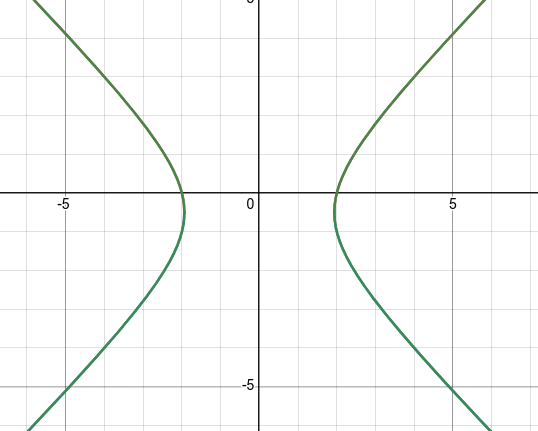
\includegraphics[scale=0.45]{fig1.png}}
	\subfigure[Graph of $y_1(x)$]{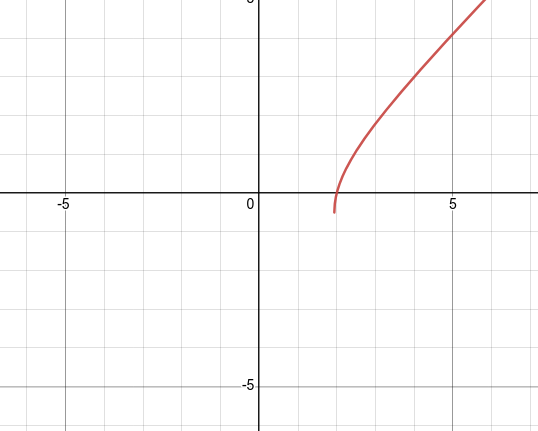
\includegraphics[scale=0.45]{fig2.png}}
	\subfigure[Graph of $y_2 (x)$]{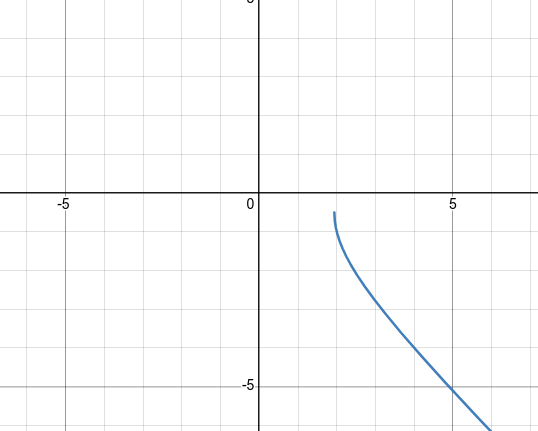
\includegraphics[scale=0.45]{fig3.png}}
	\subfigure[Graphs of $y + y^2 = x^2 - 4$ and $y_1(x)$]{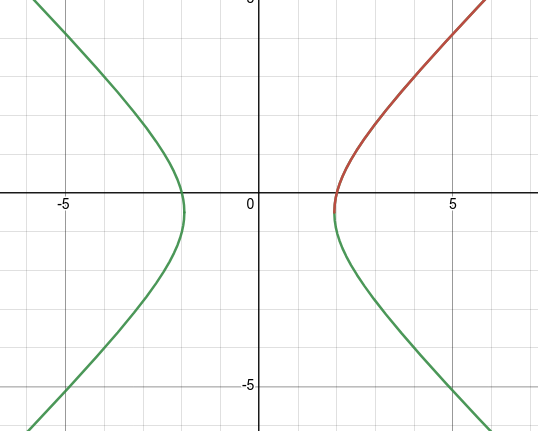
\includegraphics[scale=0.45]{fig4.png}}
	\end{figure}
	
\end{document}